% A skeleton file for producing Computer Engineering reports
% https://kgcoe-git.rit.edu/jgm6496/KGCOEReport_template

\documentclass[CMPE]{../KGCOEReport}

% The following should be changed to represent your personal information
\newcommand{\classCode}{EEEE 380}  % 4 char code with number
\newcommand{\name}{Andrei Tumbar}
\newcommand{\LabSectionNum}{1}
\newcommand{\LabInstructor}{Dr.\ Moon}
\newcommand{\TAs}{Karen Chen}
\newcommand{\exerciseNumber}{2}
\newcommand{\exerciseDescription}{Design and Simulation of NMOS Inverters}

\usepackage{tikz}
\usepackage{circuitikz}
\usetikzlibrary{calc}
\usepackage{multirow}
\usepackage{titlesec}
\usepackage{float}
\usepackage{lmodern}
\usepackage{siunitx}
\usepackage{subcaption}
\usepackage{graphicx}
\usepackage[usestackEOL]{stackengine}
\usepackage{scalerel}
\usepackage[T1]{fontenc}
\usepackage{amsmath}


\def\code#1{\texttt{#1}}

\begin{document}
    \maketitle
    \section*{Abstract}

    In this exercise, the behaviour of RTL and SEL inverters was investigated by
    simulating the circuits in SPICE. The effects of varying different parameters
    inside the load device (resistance and load transistor strength) was investigated.
    VTC curves were shown for both of the inverter types as well as plots for inverter
    response due to varying parameters. \\

    \section*{RTL Inverter}

     The resistor-transistor inverter is an inverter with a resistor load and
     transistor driver. A VTC curve was simulated in LT-SPICE.
     
     \begin{figure}[h!]
     	\centering
       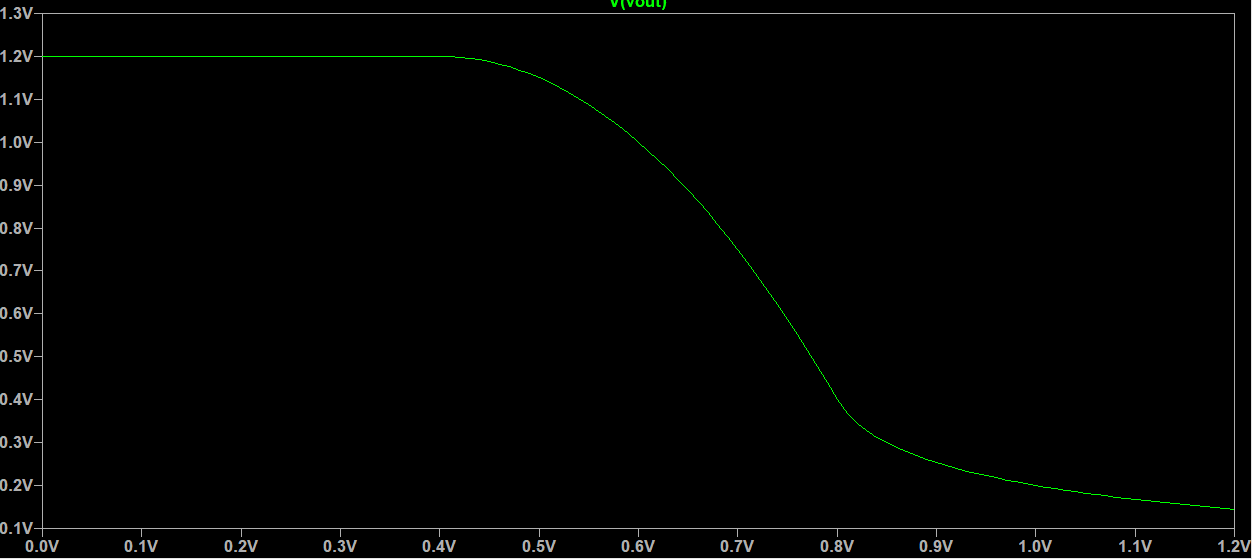
\includegraphics[width=5.5in]{img/rtl_vtc}
       \caption{Base RTL VTC curve}
       \label{fig:rtl_vtc}
	 \end{figure}

	Figure \ref{fig:rtl_vtc} shows that $V_{OH}$ will reach the $V_{DD}$ which
	is expected with the RTL inverter. $V_{OL}$ will not drop below $0.15V$ due
	to the driver strength not being strong enough to overcome the resistor load.

	To show the relationship between the $V_{OL}$ and the resistance of the load,
	three simulations were performed with varying resistances.

	\pagebreak
	
	\begin{figure}[h!]
		\centering
       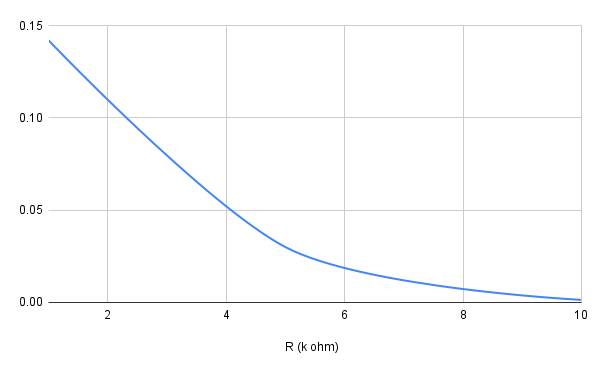
\includegraphics[width=5.5in]{img/vol_vs_r}
       \caption{$V_{OL}$ vs $R$}
       \label{fig:vol_vs_r}
	 \end{figure}

	Figure \ref{fig:vol_vs_r} shows that as the resistance increases, $V_{OL}$
	drops to near $0V$. Figure \ref{fig:vol_vs_r} shows the behaviour of the
	VTC curve in response to a change in the characteristics of the load. This
	exercise also looked at the behaviour in response to a change in the strength
	of the driver. To do this, the driver transistor's width was varied there-by
	changing its strength relative to the load.
	
	\begin{figure}[h!]
		\centering
       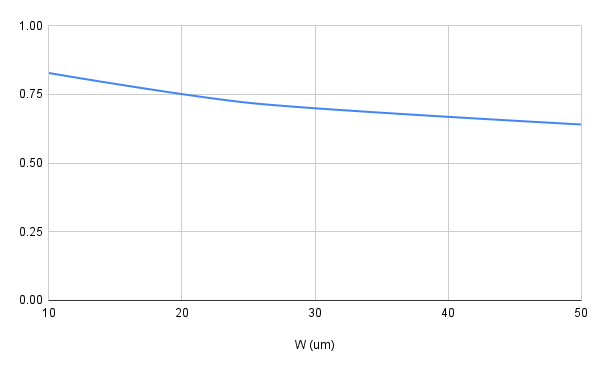
\includegraphics[width=5.5in]{img/vth_vs_w}
       \caption{$V_{th}$ vs $W$}
       \label{fig:vol_vs_w}
	 \end{figure}


    \section*{Saturated enhancement-load inverter}

    The saturated enhancement-load inverter works by wiring two enhancement
    NMOS devices in series. The drain of the load is connected to $V_{DD}$ while
    the drain of the driver is connected to the output. The driver's gate is the
    input and the load's gate is $V_{DD}$. Due to the threshold voltage of the
    load and its body effect, $V_{OH}$ will not reach $V_{DD}$ as there will always
    be a voltage drop across the load device.\\

	To show the characteristic response of the SEL inverter to the presence of
	body effect, two VTC curves were generated with $\gamma=0V^{1/2}$ and
	$\gamma=0.2V^{1/2}$.

	\begin{figure}[h!]
		\centering
       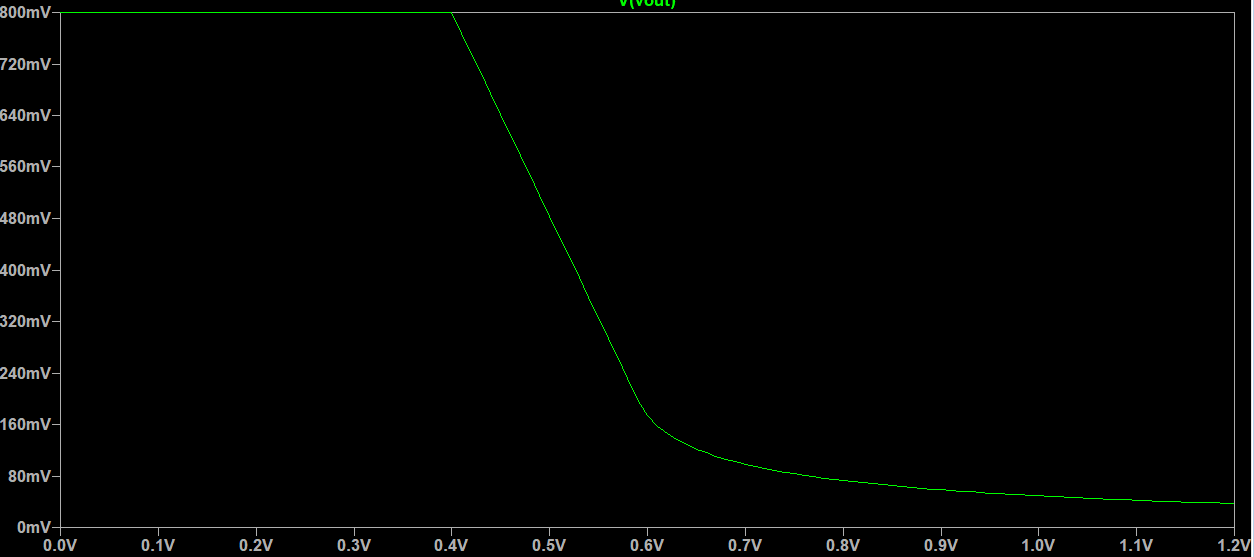
\includegraphics[width=5.5in]{img/sel_no_body}
       \caption{SEL VTC without body effect on load NMOS}
       \label{fig:no_body}
	 \end{figure}

	\begin{figure}[h!]
		\centering
       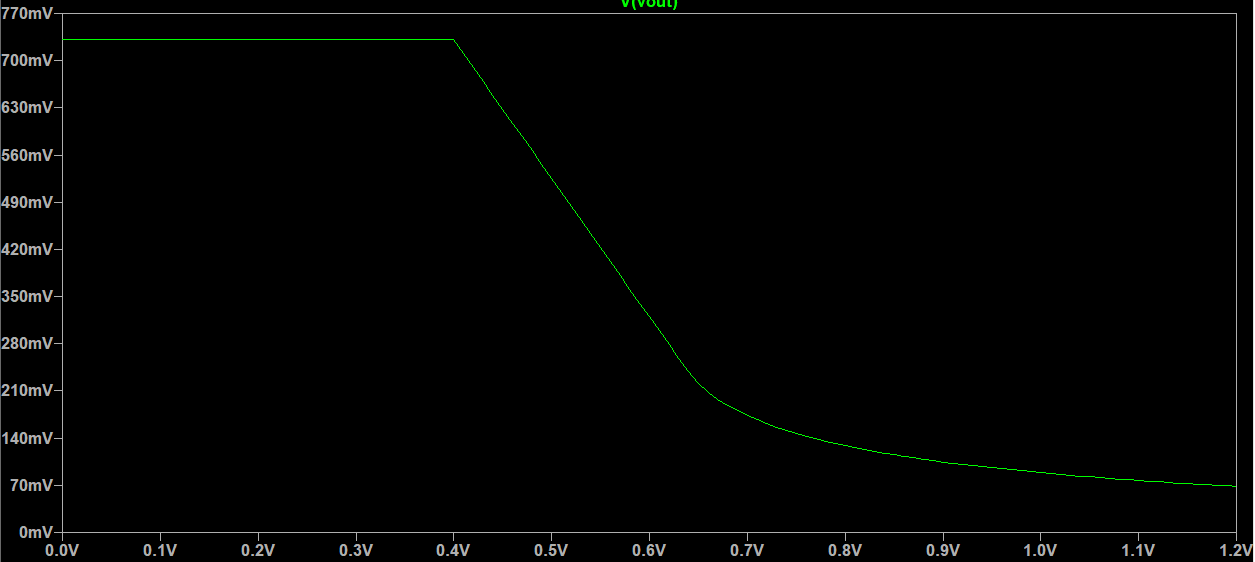
\includegraphics[width=5.5in]{img/sel_body}
       \caption{SEL VTC with body effect $\gamma=0.2V^{1/2}$ on load NMOS}
       \label{fig:body}
	 \end{figure}

	The SEL inverter will not reach a $V_{OH}$ equal to its high supply $V_{DD}$.
	Without body effect, this voltage reach $0.8V$ with a $V_{DD}$ of $1.2V$.
	With body effect, the voltage only reaches $0.731V$. This is expected as the
	response due to body effect should decrease $V_{OH}$ according to the prelab
	calculations. Due to $V_{OH}$ dropping in response to body effect, $V_{OL}$
	is expected to rise as the input voltage for a low output will not be lower.
	As expected, $V_{OL}$ rises from $0.073V$ to $0.091V$ 
	when $\gamma=0.2V^{1/2}$.\\

	In addition to body effect, the SEL inverter's VTC curve will respond to
	changes in the relative strength between the driver and load.
	This relationship is denoted as $K_r$ and is equavalent to
	$k_{driver} / k_{load}$. This ratio may be changed by fixing $(\frac{W}{L})_1$
	and varying $(\frac{W}{L})_2$. A plot showing the effect of $K_r$ on $V_{OL}$
	and $V_{th}$ was generated.
	
	\begin{figure}[h!]
		\centering
       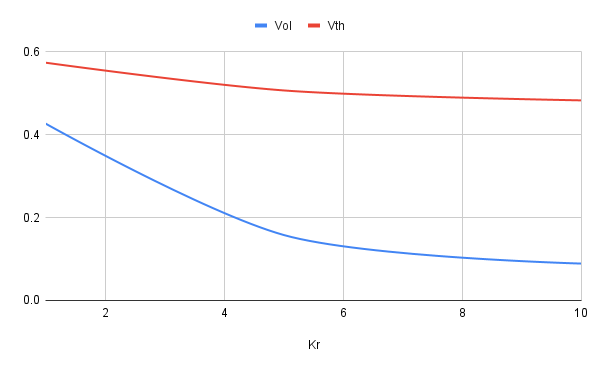
\includegraphics[width=5.5in]{img/vol_vth_kr.png}
       \caption{Effect of $K_r$ on $V_{OL}$ and $V_{th}$ of SEL inverter}
       \label{fig:kr}
	 \end{figure}

	Figure \ref{fig:kr} shows expected results. As the strength of the driver
	increases relative to the load ($k_{driver} \propto K_r$), the output low
	decreases. This is because the driver is able to pull the output lower.

	\section*{Conclusion}
	This exercise investigated the RTL and SEL inverters by comparing their
	operations while varying characterics of each device. The behaviour of the
	RTL inverter was shown while varying the resistance of the load as well as
	the width of the driver NMOS device. The behaviour of SEL inverter was
	shown while by showing the VTC curve due to body effect on the load
	device as well as varying the relative strength of the driver to load $K_r$.
	Both the RTL and SEL inverters showed expected behavioural response in the
	simulations when comparing to the prelab calculations. The goals of the this
	exercise were reached as the circuits were successfully simulated and the
	prelab calculations were supported by the simulation results.

\end{document}
